\documentclass[12pt]{report}
\hbadness=100000%
\usepackage[margin=1in]{geometry}
\setlength{\parskip}{5pt}
\usepackage{xurl}
\usepackage{amsmath}
\usepackage{mathtools}
\usepackage{graphicx}
\usepackage{float}
\usepackage{textcomp}
\usepackage{gensymb}
\renewcommand{\bibname}{References}

\title{ECE 496 - Silicon Integrated Circuit Design Technology Lab 4: Photolithography\\ Spring 2026, Lab Section B}
\author{Gianni Avilan-Losee}
\date{\today}
\begin{document}
\maketitle
\setcounter{chapter}{4}
\setcounter{section}{0}
\section{Objectives}

This lab's objective was to demonstrate the process of silicon wafer photolithography, including the baking, mask alignment, UV light exposure, and photoresist development steps. 

\section{Background}

The photolithography process varies widely across different manufacturers and devices; the process used in this lab consisted of the following steps: wafer cleaning, prebake, photoresist application, soft bake, UV exposure, development, hard bake. The goal of the photolithography process is subtractive; that is, to cover the wafer in a photoresist material, which may be removed in a specific pattern, to then dope or otherwise change the substrate material. Then, the photoresist is washed away to begin the process anew\cite{textbook}.

\section{Procedure}

After following proper gowning and cleanroom procedure, and entering the lab, the 100mm wafers were coated in a pre-prepared photoresist material manually, using a pipette, at which point the wafer was spin coated for 60 seconds at 2000 RPM. This process was done twice, with two separate, chemically different photoresist materials. 

Following this, the wafers were "soft baked" at \(110 \degree \mathrm{C}\) for one minute. The wafer was then loaded onto the mak aligner, and the UV light source was activated for 30 seconds to pattern the photoresist.

Then, the wafer was carefully inserted into a developer solution to wash away the weakened photoresist, and left for roughly five minutes, after which it was rinsed using DI water. Finally, a post-bake was performed at \(110 \degree \mathrm{C}\) for five minutes.

Then, the wafers were transferred to another bay for inspection. 

Using an optical surface profiler, a three-dimensional plot of the wafer was generated digitally.

The following are images of the above-described procedures.

\begin{figure}[H]
  \centering
  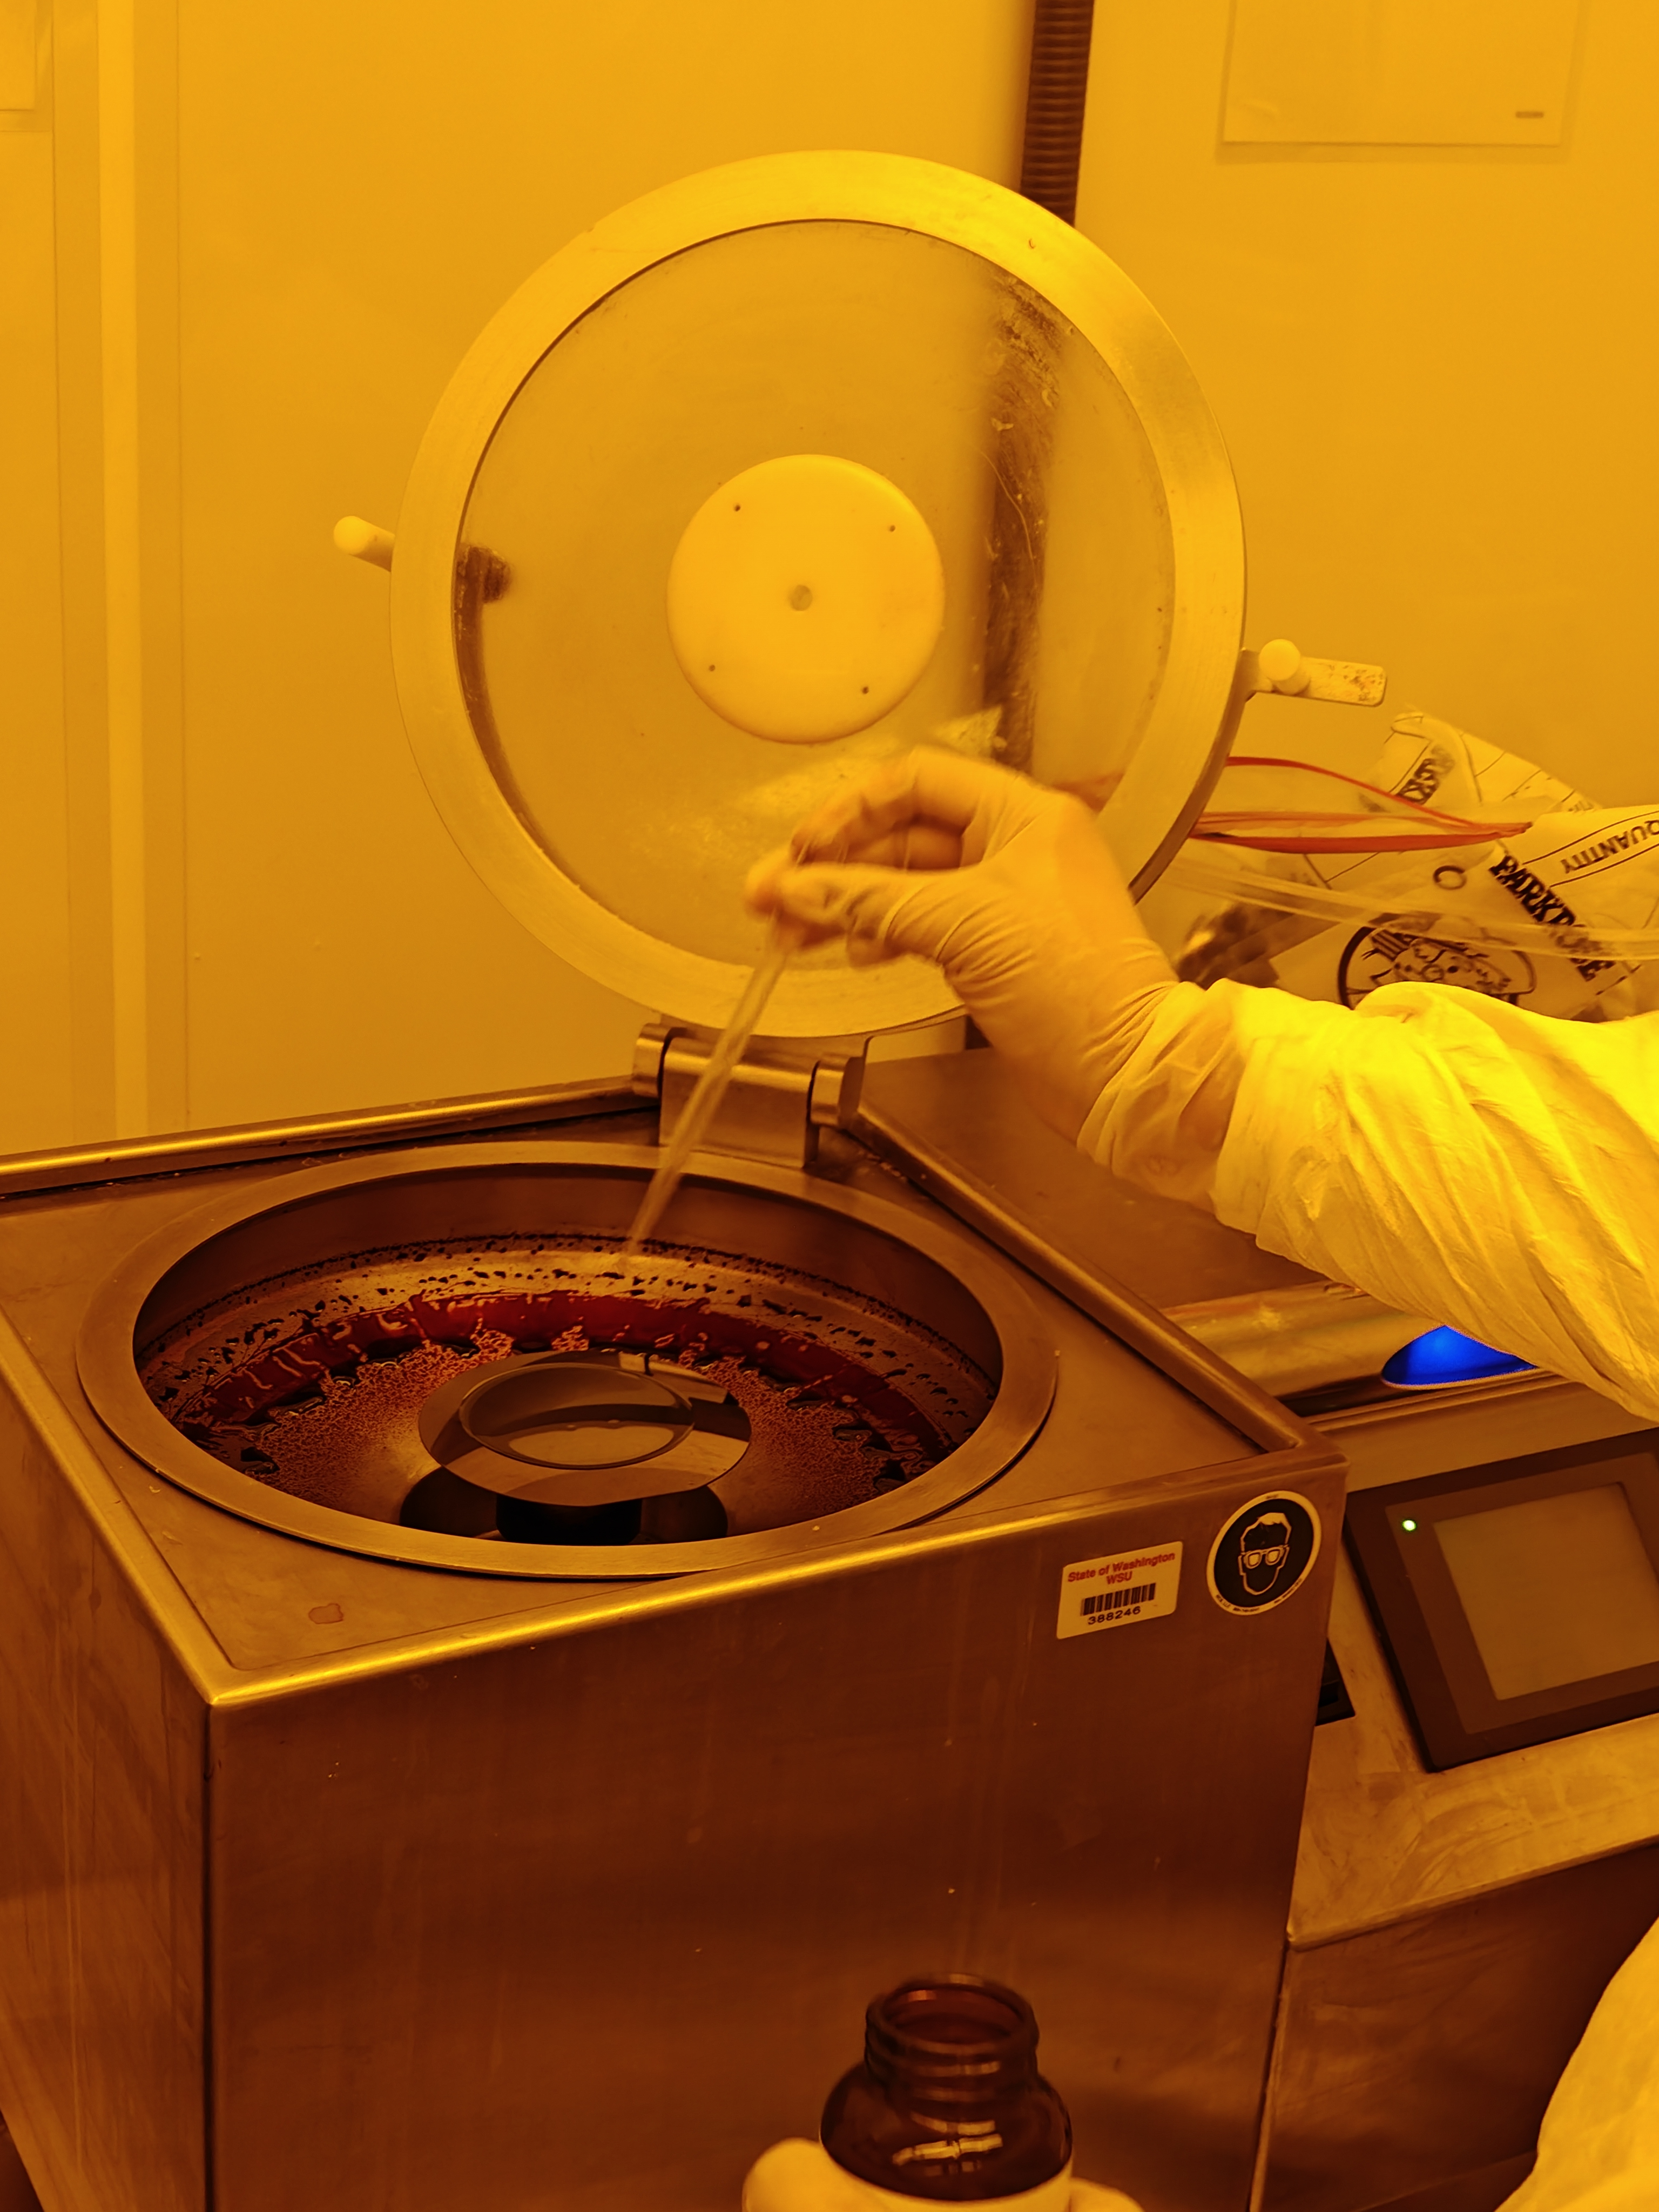
\includegraphics[width=0.8\textwidth]{lab-report-4_fig-1.jpg}
  \caption{Photoresist application prior to spin coating}
  \label{fig:spincoat}
\end{figure}

\begin{figure}[H]
  \centering
  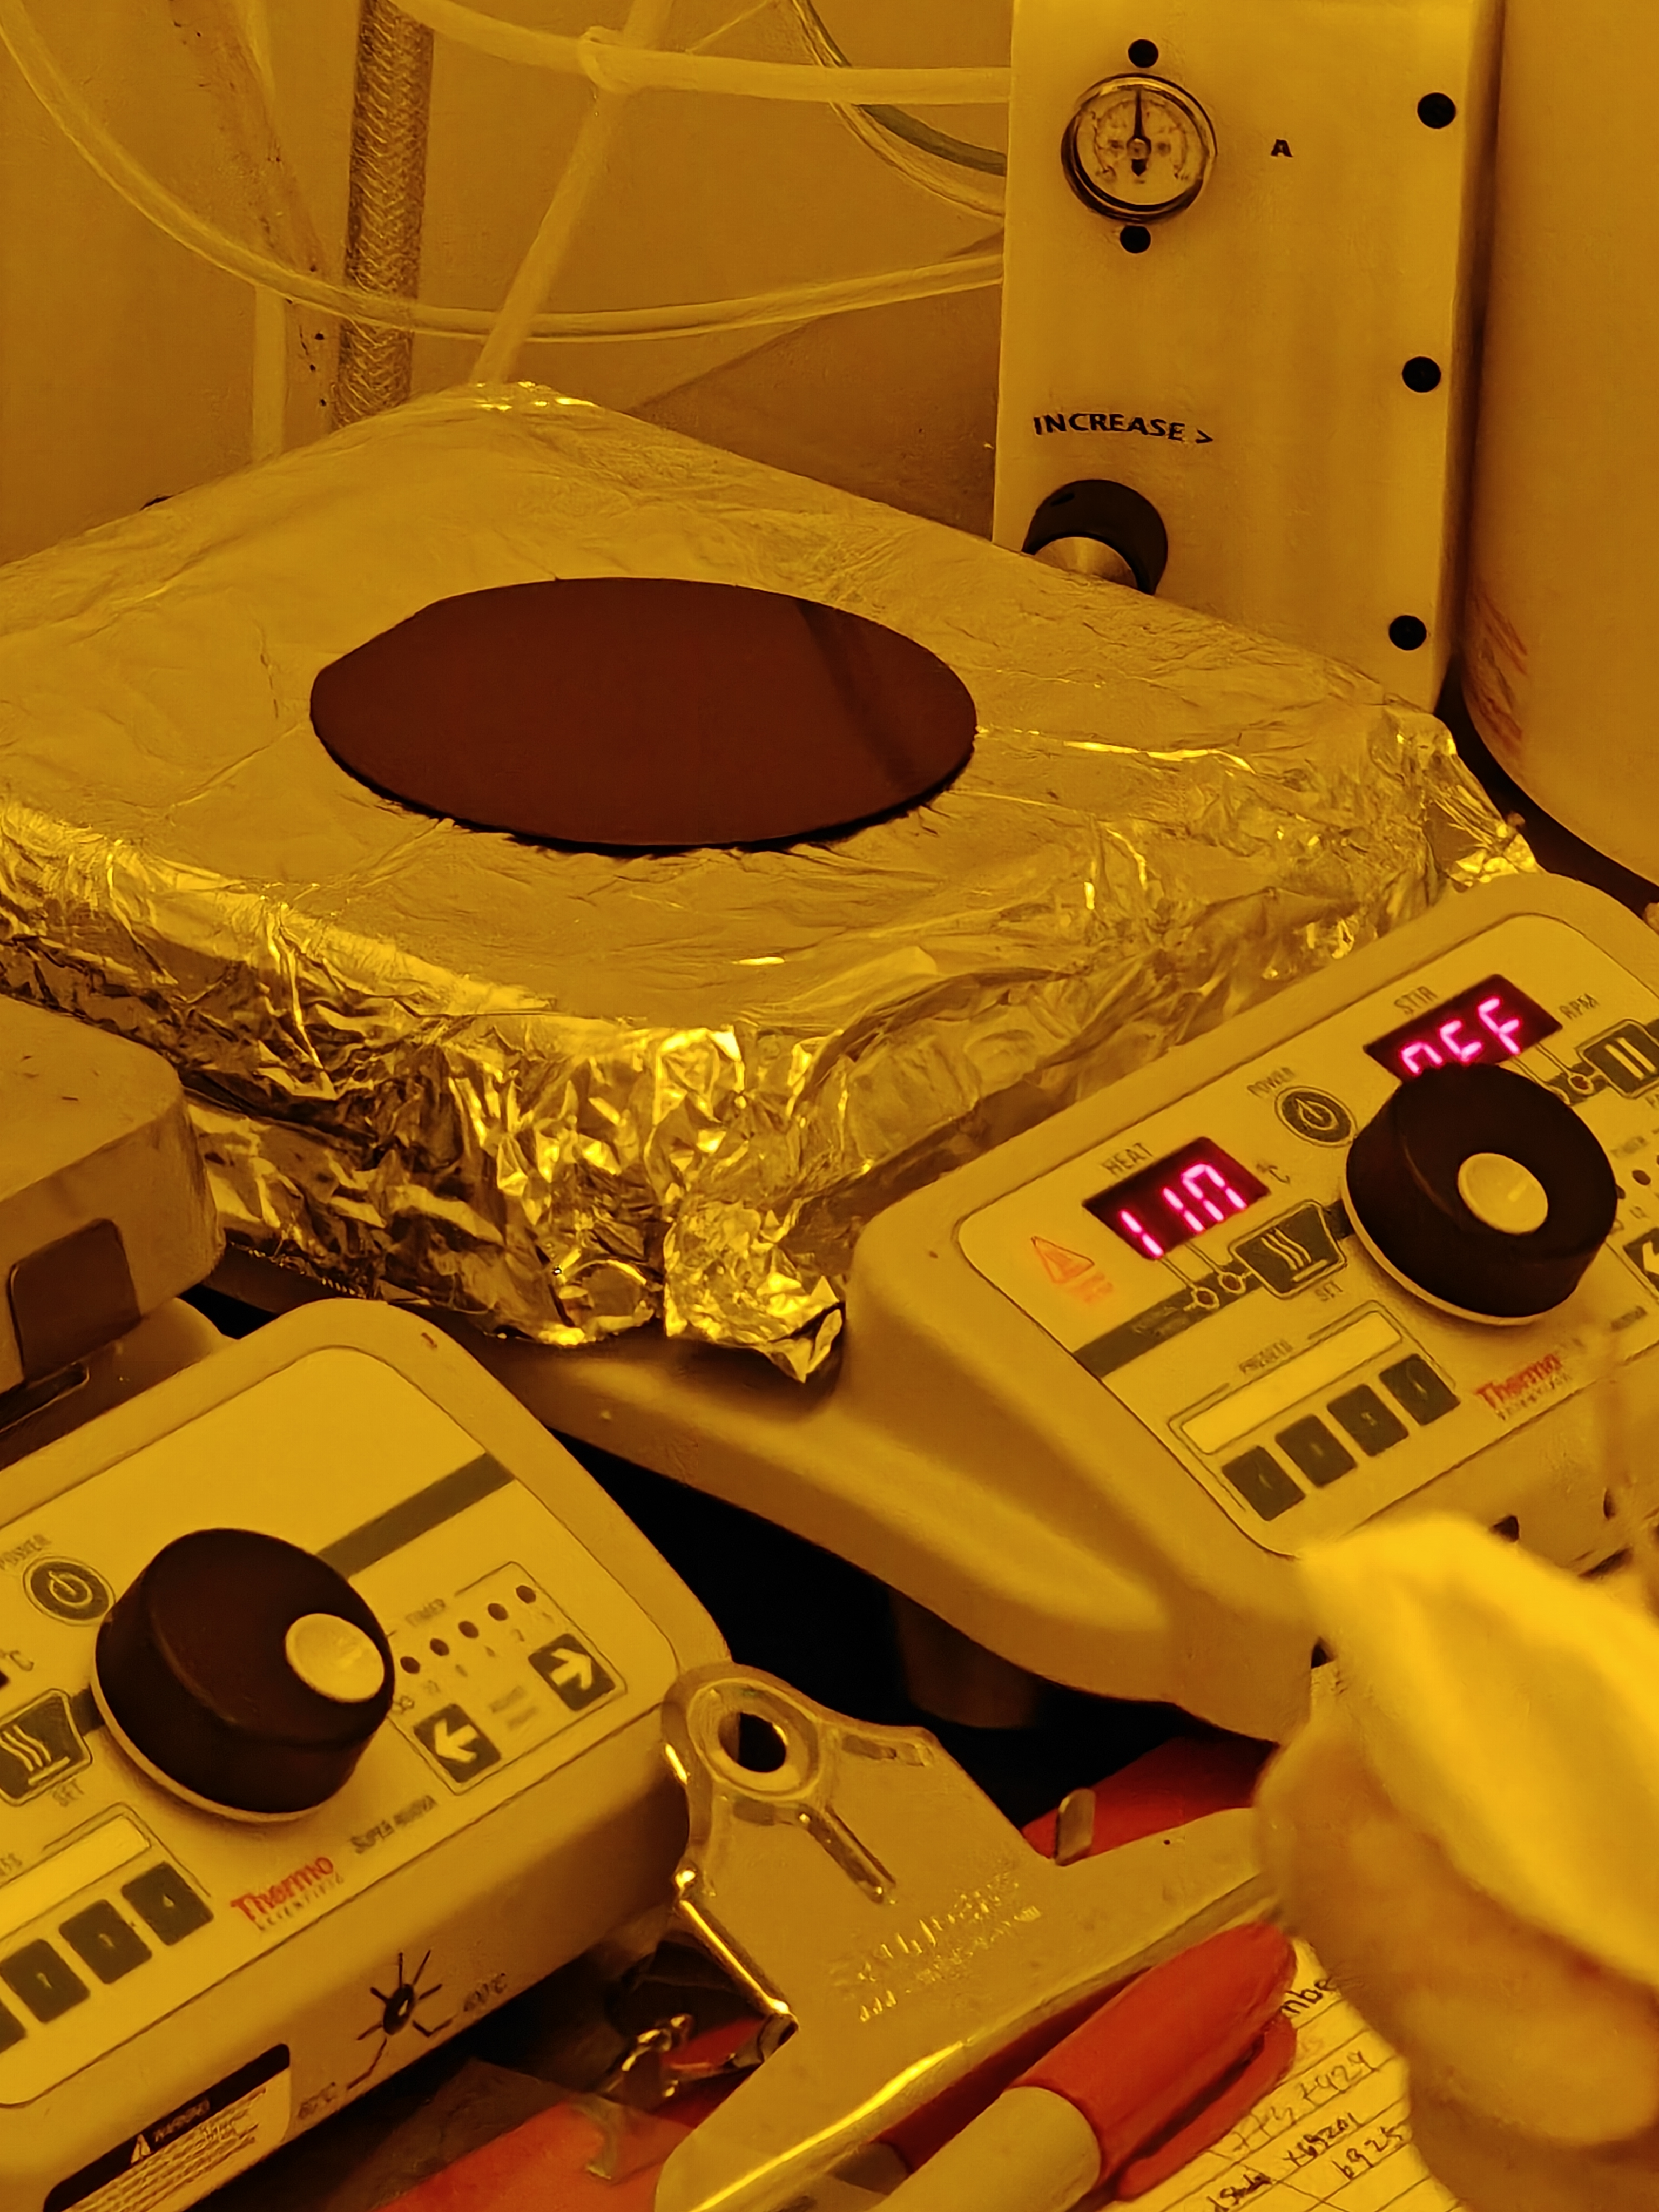
\includegraphics[width=0.8\textwidth]{lab-report-4_fig-2.jpg}
  \caption{Soft baking the wafer}
  \label{fig:cookin}
\end{figure}

\begin{figure}[H]
  \centering
  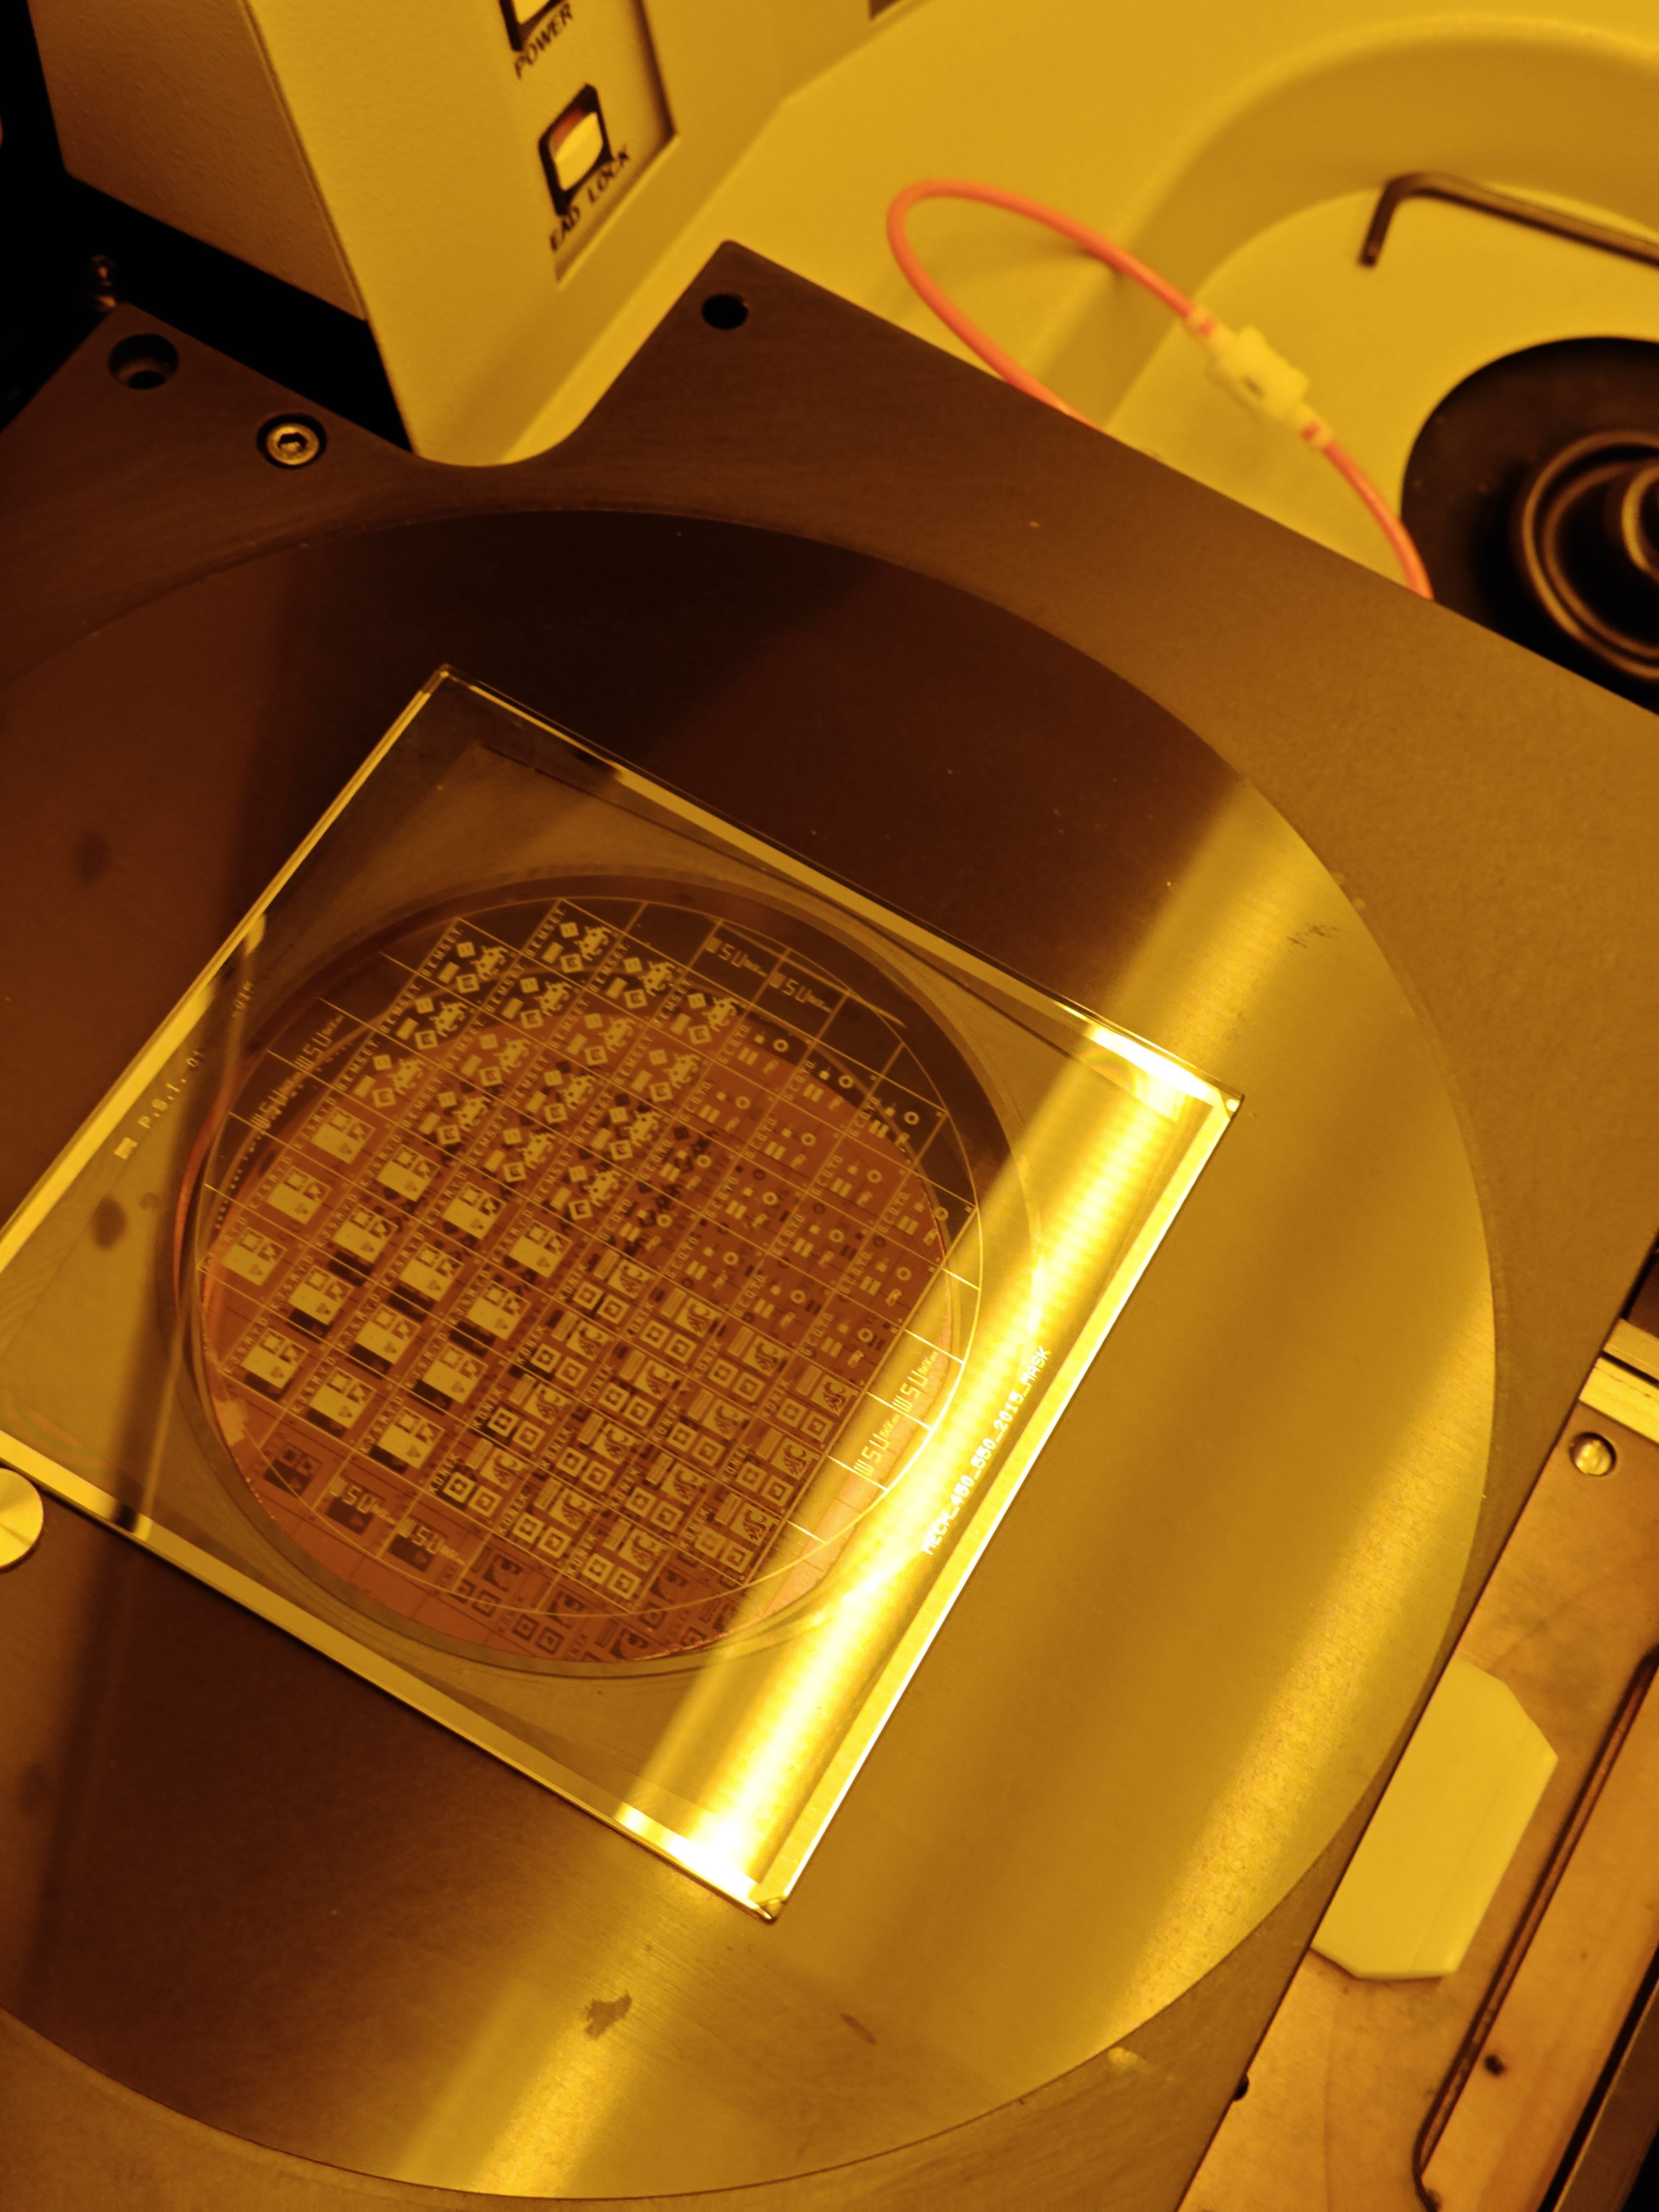
\includegraphics[width=0.8\textwidth]{lab-report-4_fig-3.jpg}
	\caption{The result of UV light exposure and development}
  \label{fig:final}
\end{figure}

\begin{figure}[H]
  \centering
  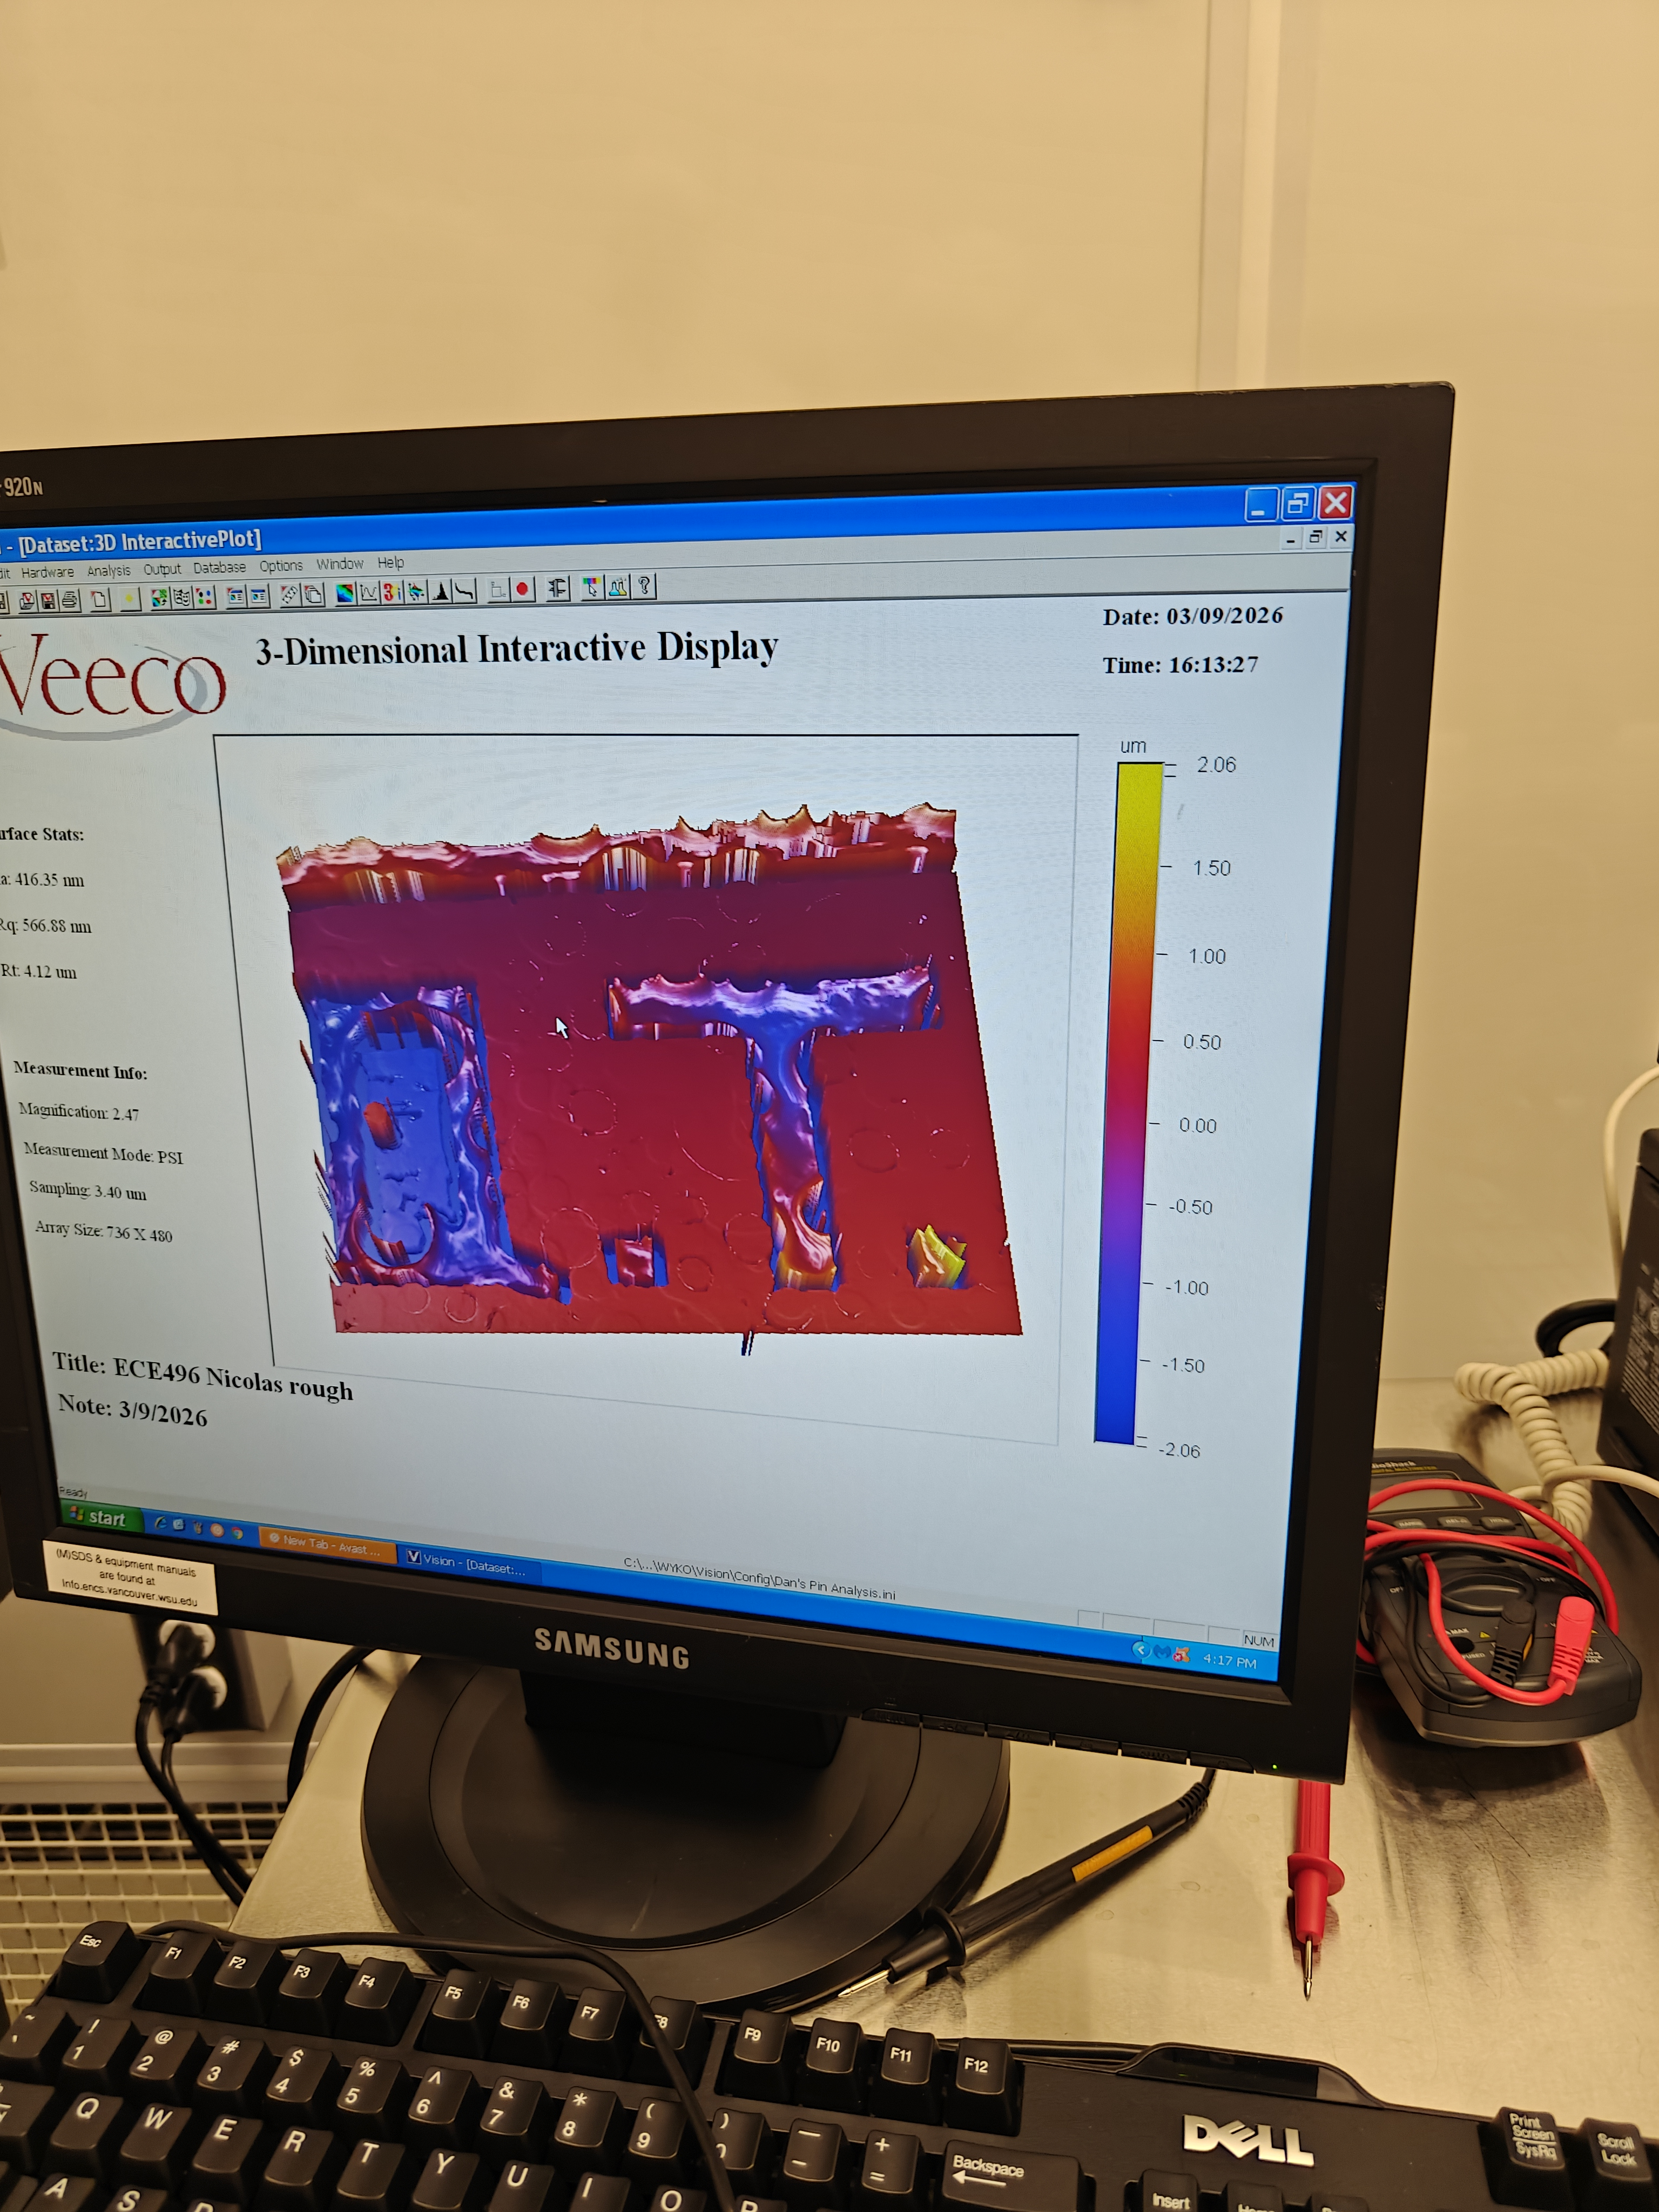
\includegraphics[width=0.8\textwidth]{lab-report-4_fig-4.jpg}
	\caption{The resulting 3D plot of the wafer's surface}
  \label{fig:plot}
\end{figure}

\section{Results and Discussion}

Though numerical results of the experiment were not captured, the resultant 3D plot showed an average difference of roughly \(2 \mathrm{\micro m}\), along with some unwanted artifacts likely produced by imprecisions in the mask alignment process, or other environmental variables.

\section{Conclusion}

In conclusion, this lab demonstrated the photolithography process and its drawbacks as well as the potential for errors and unwanted artifacts when the process is not performed with attention to detail.

\begin{thebibliography}{4}
	\bibitem{textbook} Jaeger, R. (2001). \textit{Introduction to Microelectronic Fabrication: Volume 5 (Modular Series on Solid State Devices} (2nd ed.). Pearson.
\end{thebibliography}

\end{document}

